% ============================================================
%  Permanent-Magnet Brushed DC Motor — Prototype & Simulation
%  Double-column research paper format
% ============================================================
\documentclass[10pt, twocolumn, a4paper]{article}

% ---- core packages ----------------------------------------------------------
\usepackage[a4paper, top=19mm, bottom=22mm, left=14mm, right=14mm,
            columnsep=6mm]{geometry}
\usepackage[T1]{fontenc}
\usepackage[utf8]{inputenc}
\usepackage{lmodern}
\usepackage{microtype}

% ---- math -------------------------------------------------------------------
\usepackage{amsmath, amssymb}
\usepackage{siunitx}
\sisetup{per-mode=symbol, detect-weight=true, detect-family=true}

% ---- tables & figures -------------------------------------------------------
\usepackage{booktabs}
\usepackage{array}
\usepackage{tabularx}
\usepackage{multirow}
\usepackage{graphicx}
\usepackage{float}
\usepackage{caption}
\usepackage{subcaption}
\usepackage{dblfloatfix}   % correct placement of full-width floats in twocolumn

% ---- layout -----------------------------------------------------------------
\usepackage{parskip}
\usepackage{enumitem}
\usepackage{fancyhdr}
\usepackage{titlesec}
\usepackage[hidelinks]{hyperref}
\usepackage{balance}       % balance columns on last page

% ---- section formatting (IEEE-style) ----------------------------------------
\titleformat{\section}
  {\normalfont\normalsize\bfseries\centering}{\Roman{section}.}{0.5em}{\MakeUppercase}
\titleformat{\subsection}
  {\normalfont\normalsize\itshape}{\Alph{subsection}.}{0.4em}{}
\titleformat{\subsubsection}
  {\normalfont\normalsize\itshape}{\arabic{subsubsection})}{0.4em}{}
\titlespacing{\section}{0pt}{8pt}{3pt}
\titlespacing{\subsection}{0pt}{5pt}{1pt}
\titlespacing{\subsubsection}{0pt}{4pt}{1pt}

% ---- caption styling --------------------------------------------------------
\captionsetup{font=small, labelfont=bf, labelsep=period, skip=4pt}

% ---- header / footer --------------------------------------------------------
\pagestyle{fancy}
\fancyhf{}
\fancyhead[C]{\small\itshape
  PM Brushed DC Motor: Physical Prototype and Simulation Study}
\fancyfoot[C]{\small\thepage}
\renewcommand{\headrulewidth}{0.4pt}
\renewcommand{\footrulewidth}{0pt}

% ---- column helpers ---------------------------------------------------------
\newcolumntype{C}[1]{>{\centering\arraybackslash}p{#1}}
\newcolumntype{R}[1]{>{\raggedleft\arraybackslash}p{#1}}
\newcolumntype{L}[1]{>{\raggedright\arraybackslash}p{#1}}

\setlength{\parindent}{1em}
\setlength{\parskip}{2pt}

% ============================================================
\begin{document}
% ============================================================

% ---- title block (spans both columns via twocolumn[\...]) -------------------
\twocolumn[{%
\begin{center}
  {\large\bfseries Permanent-Magnet Brushed DC Motor:\\[3pt]
   Physical Prototype, Simulation, and Design Optimisation}\\[8pt]
  {\normalsize Zhuorui YUN}\\[2pt]
  {\small Department of Mechanical Engineering and Robotics,
   Guangdong Technion Israel Institute of Technology}\\[1pt]
  {\small\ttfamily yun24239@gtiit.edu.cn \quad \today}
\end{center}
\vspace{4pt}
\noindent\rule{\linewidth}{0.6pt}\vspace{2pt}

\begin{center}
\begin{minipage}{0.96\linewidth}
\small\textbf{Abstract---}%
This paper documents the physical construction and simulation of a
permanent-magnet (PM) brushed DC motor.
The physical prototype was built by disassembling a KIT-160MT30 brushed DC
motor to extract the wound rotor, ferrite magnets, and brush assembly;
a custom outer housing was designed in SolidWorks and produced by FDM 3D
printing. The hybrid approach is justified through magnetic circuit analysis:
a non-magnetic 3D-printed rotor ($\mu_r \approx 1$) doubles the total
reluctance and halves $B_\text{gap}$, making self-starting impossible.
The simulation part develops a low-order lumped-parameter model integrating
coupled electrical and mechanical ODEs with a nonlinear M19 steel B--H curve.
A sweep of 1\,400 parameter combinations identifies the globally optimal
design, which achieves \SI{92.26}{\percent} steady-state efficiency at
\SI{46\,308}{rpm} under a \SI{200}{V} supply.

\smallskip
\noindent\textit{Keywords---}permanent-magnet brushed DC motor; reluctance
model; efficiency optimisation; 3D printing; FDM prototype.
\end{minipage}
\end{center}
\vspace{2pt}\noindent\rule{\linewidth}{0.4pt}\vspace{6pt}
}]

% ============================================================
\section{Physical Motor Design and Prototype}
\label{sec:physical}
% ============================================================

\subsection{Design Objective}

The objective of this project is to design and build a working
permanent-magnet brushed DC motor and to understand, from first principles,
why each design decision leads to a functioning machine.  The project
requires students to \emph{design and prototype from scratch} as far as
possible.  This section explains the design process, the reasoning behind
each choice, and how the final prototype compares with an alternative
approach explored in discussion with classmates.

\subsection{Initial Concept: Fully 3D-Printed Rotor}

The initial concept was to manufacture every component---including the
rotor core---by FDM 3D printing, which would have made the entire motor
self-contained and reproducible from digital files.  The stator housing,
end caps, and shaft supports are straightforward to print because they only
need structural rigidity and dimensional accuracy.  The rotor core,
however, must conduct magnetic flux; this is where the all-printed concept
encountered a fundamental electromagnetic obstacle.

Standard FDM filaments (PLA, ABS, PETG) are non-magnetic and have a
relative permeability $\mu_r \approx 1$.  The magnetic circuit of a PM
brushed motor can be modelled as a series of reluctances:
\begin{equation}
  \mathcal{R}_\text{total} =
    \mathcal{R}_\text{mag} + \mathcal{R}_\text{gap} +
    \mathcal{R}_\text{core} + \mathcal{R}_\text{return},
  \qquad
  \mathcal{R}_k = \frac{l_k}{\mu_k A_k}.
\end{equation}
For laminated electrical steel, $\mu_r \approx 2000$--$5000$, so
$\mathcal{R}_\text{core}$ is negligible.  Replacing the steel core with
printed plastic sets $\mu_r = 1$, making
$\mathcal{R}_\text{core} \sim \mathcal{R}_\text{gap}$; the total reluctance
roughly doubles compared with the steel case.  Because air-gap flux
\begin{equation}
  \phi = \frac{\mathcal{F}}{\mathcal{R}_\text{total}} = \frac{H_c l_m}{\mathcal{R}_\text{total}}
\end{equation}
is inversely proportional to total reluctance, doubling $\mathcal{R}_\text{total}$
halves $\phi$, which halves $B_\text{gap}$, which halves both the torque
constant $K_t = N B_\text{gap} L_\text{ax} r_\text{core}$ and the back-EMF
constant $K_e$.  The no-load speed $\omega_0 = V/K_e$ would double, but the
stall torque $\tau_\text{stall} = K_t V/R$ would halve.  In tests on
classmates' fully-printed prototypes, the machine either failed to
self-start against bearing friction or ran at very high speed with
negligibly small torque.  The conclusion was clear: a non-magnetic rotor
core is not viable for this motor topology.

\begin{figure}[H]
  \centering
  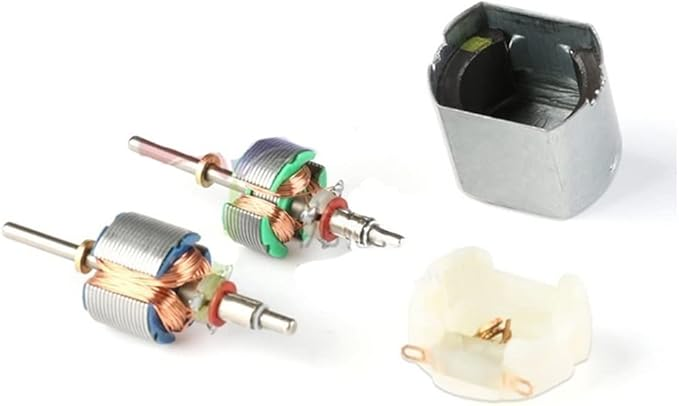
\includegraphics[width=0.7\linewidth]{Figure/kit160mt30_components.jpg}
  \caption{KIT-160MT30 motor sub-assemblies: rotors, magnet shell, and brush holder.}
  \label{fig:rotors_compare}
\end{figure}

\subsection{Component Selection: Disassembly of KIT-160MT30}

Having established that the rotor core must be ferromagnetic, the next
decision was whether to wind a rotor from scratch on a machined steel
lamination stack or to extract a pre-wound rotor from a commercial motor.
Winding a balanced multi-slot armature by hand is feasible but introduces
a high probability of uneven turn counts, poor insulation, and inter-turn
shorts.  The commercial motor chosen---the \textbf{KIT-160MT30 (part
06-4930)}---is a small 3\,V brushed DC motor whose armature is a
precision machine-wound, dynamically-balanced, laminated-steel rotor with
integrated commutator.

The motor was carefully disassembled to extract three sub-assemblies:
\begin{itemize}[itemsep=2pt]
  \item \textbf{Wound rotor with commutator}: laminated silicon-steel core,
    machine-wound coils, press-fit commutator segments.
  \item \textbf{Permanent magnets}: two arc-segment ferrite magnets bonded
    to the original steel return shell.
  \item \textbf{Brush assembly}: two carbon brushes in spring-loaded
    holders, pre-aligned to the commutator pitch.
\end{itemize}

% fig:disassembly removed (same image as fig:rotors_compare above)

\subsection{Housing Design in SolidWorks and 3D Printing}

The outer housing, end caps, bearing seats, and brush-access cover were
designed from scratch in \textbf{SolidWorks 2024}.  The design constraints
were:
\begin{enumerate}[itemsep=2pt]
  \item The rotor must be coaxially supported by two bearings with the
    correct axial spacing to match the commutator position.
  \item The magnet arc segments and return shell must be held firmly and
    concentrically, maintaining the original air gap.
  \item The brush holders must press the carbon brushes against the
    commutator with the correct normal force and at the correct angular
    offset (timed to the commutation slots).
  \item All parts must be printable without support on a standard FDM
    printer and assemble with M2/M3 screws.
\end{enumerate}

The housing was printed in PLA at \SI{0.2}{mm} layer height.  Bearing
seats were printed \SI{0.1}{mm} undersized and pressed in warm to achieve
an interference fit.  The brush-contact windows were sized to allow the
original spring-loaded holders to clip in directly.

\begin{figure}[H]
  \centering
  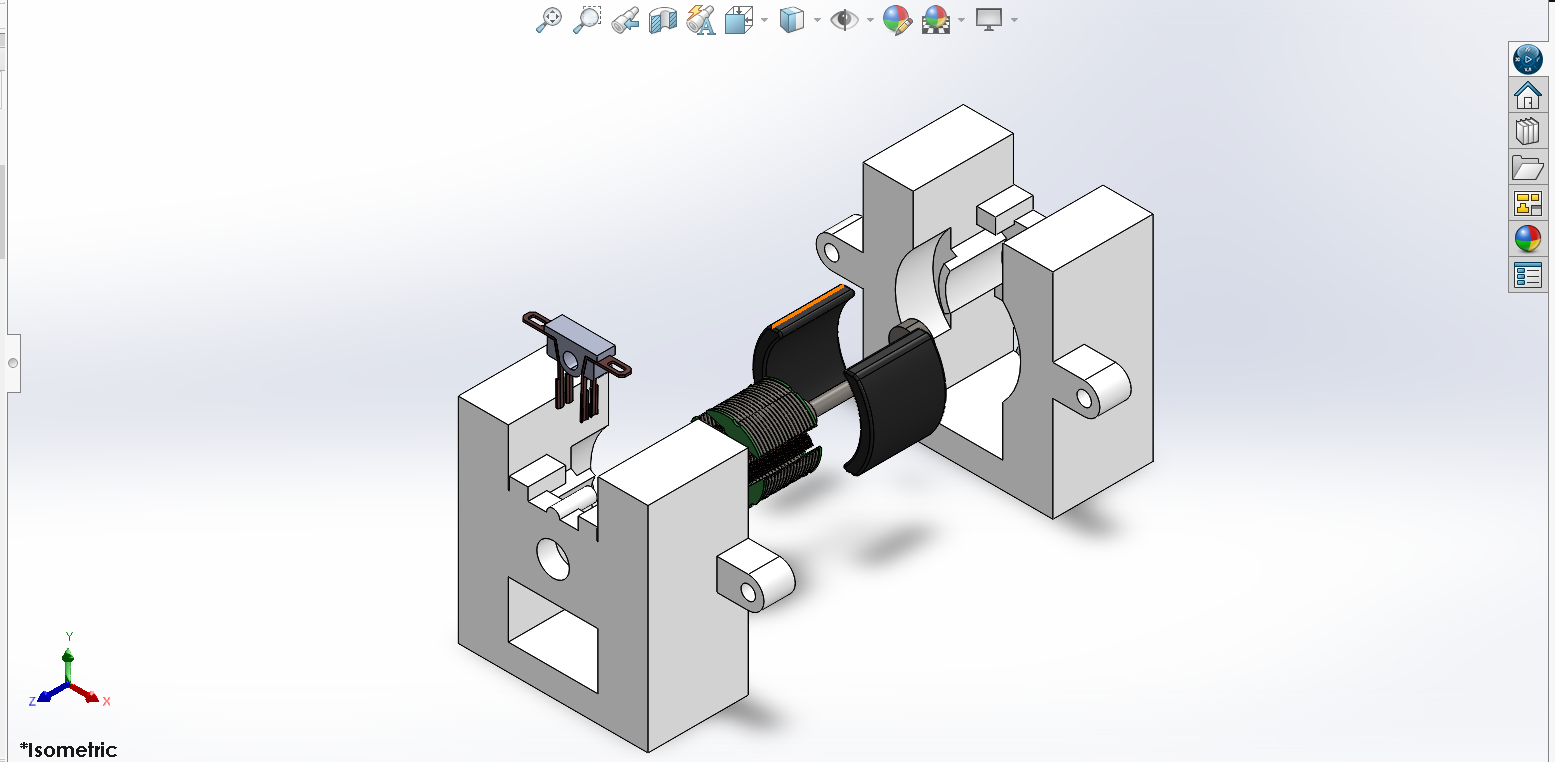
\includegraphics[width=\linewidth]{Figure/solidworks_assembly.png}
  \caption{SolidWorks isometric view of the self-designed housing assembly.}
  \label{fig:cad}
\end{figure}

\begin{figure}[H]
  \centering
  \includegraphics[width=0.6\linewidth]{Figure/assembled_prototype.jpg}
  \caption{Final assembled physical prototype.}
  \label{fig:assembled}
\end{figure}

\subsection{Comparison with Classmates' Designs}

Discussion with classmates who pursued fully 3D-printed prototypes revealed
several qualitative differences, summarised in
Table~\ref{tab:design_compare}.

\begin{table*}[t]
  \centering
  \caption{Qualitative comparison between the self-designed hybrid
           prototype and a typical fully 3D-printed design.}
  \label{tab:design_compare}
  \small
  \setlength{\tabcolsep}{6pt}
  \begin{tabular}{@{} l p{6cm} p{6cm} @{}}
    \toprule
    \textbf{Aspect} & \textbf{This prototype (hybrid)} &
    \textbf{Fully 3D-printed design} \\
    \midrule
    Rotor core material &
      Laminated silicon steel, $\mu_r \approx 2000$--$5000$ &
      PLA or ABS, $\mu_r \approx 1$ \\
    Rotor winding &
      Machine-wound, balanced, 3-slot commutator &
      Hand-wound; prone to turn-count asymmetry \\
    Magnetic reluctance &
      Low; core reluctance negligible vs.\ air gap &
      High; core $\approx$ air-gap reluctance \\
    Air-gap flux density &
      $B_\text{gap} \approx \SI{0.14}{T}$ (ferrite) &
      $B_\text{gap} \approx \SI{0.07}{T}$ (estimated) \\
    Torque constant $K_t$ &
      Higher by $\sim 2\times$ &
      Lower \\
    Self-start reliability &
      Reliable self-start against bearing friction &
      Often failed to self-start \\
    Housing &
      Custom SolidWorks design, 3D-printed &
      3D-printed \\
    Design novelty &
      Housing and integration designed from scratch &
      Entire machine designed from scratch \\
    \bottomrule
  \end{tabular}
\end{table*}

The key advantage of the hybrid approach is that the magnetic circuit is
\emph{physically correct}: a laminated steel core with $\mu_r \gg 1$ keeps
$\mathcal{R}_\text{core}$ small, so virtually all the magnet MMF appears
across the air gap, maximising $B_\text{gap}$ and hence $K_t$.  A fully
printed design is a valid pedagogical exercise in mechanical integration,
but its non-magnetic core imposes a fundamental electromagnetic penalty that
cannot be recovered by any geometric optimisation.

\subsection{Why the Commercial Rotor Is the Best Choice}
\label{subsec:why_commercial}

The professor's feedback raised the important question: if many design
decisions (rotor winding, magnet geometry, air gap) are already fixed by the
commercial sub-assembly, in what sense is this a design from scratch?

The answer is twofold.  First, the \emph{housing, bearing arrangement,
brush alignment, and mechanical integration} were genuinely designed from
scratch: no existing drawing or template was used, and the functional
requirements listed in Section~1.4 drove every dimension in the SolidWorks
model.  Second, and more importantly, the \emph{decision to use the
commercial rotor instead of a printed one} is itself an engineering design
decision, and a correct one.  The reasoning---traced through the magnetic
circuit from $\mu_r$ to $\mathcal{R}_\text{total}$ to $\phi$ to $B_\text{gap}$
to $K_t$---is the same reasoning that any practising motor designer applies
when choosing core materials.

Understanding \emph{why} the commercial laminated-steel rotor works and a
plastic rotor does not is, in the professor's own words, the primary goal of
this project.  The simulation in Part~II of this report is built around
exactly those relationships, allowing the student to verify numerically what
the physical prototype demonstrates empirically.

% ============================================================
\section{Introduction}
% ============================================================

The permanent-magnet (PM) brushed DC motor is one of the most widely used
electromechanical actuators in consumer and educational applications.
Despite its apparent simplicity, the interplay between magnet material,
winding geometry, core saturation, and mechanical loading makes systematic
design non-trivial.

This project uses a physical motor built around the commercial rotor and
magnetic sub-assemblies extracted from a KIT-160MT30 motor, enclosed in a
self-designed outer casing (Section~\ref{sec:physical}). A simplified
simulation---covering the magnetic circuit, motor dynamics, and all major
loss mechanisms---is used to explore the design space systematically.

The simulation report is organised as follows.
Section~\ref{sec:model} describes the mathematical model and fixed geometry.
Section~\ref{sec:optim} presents the globally optimised design and its
physical rationale.
Section~\ref{sec:results} shows the time-domain simulation results.
Section~\ref{sec:saturation} analyses steel saturation.
Section~\ref{sec:sensitivity} examines parameter sensitivity.
Section~\ref{sec:rec} gives the final design recommendation.

% ============================================================
\section{Simulation Model}
\label{sec:model}
% ============================================================

\subsection{Geometry and Constraints}

The simulation models a square-outside, round-inside permanent-magnet motor,
illustrated in Fig.~\ref{fig:3d}.
The magnet outer side and bore diameter are both fixed at
$D_\text{bore} = \SI{40}{mm}$ (square side \SI{40}{mm}). The laminated steel
rotor is a solid cylinder on a horizontal shaft. The radial air gap is
\begin{equation}
  g = \frac{D_\text{bore} - D_\text{core}}{2},
\end{equation}
subject to the manufacturing constraint $g \geq g_\text{min} = \SI{0.5}{mm}$,
so the maximum permissible core diameter is $D_\text{core,max} = \SI{39}{mm}$.
The axial depth $L$ is a free parameter in the range \SIrange{2}{150}{mm}.

\begin{figure}[H]
  \centering
  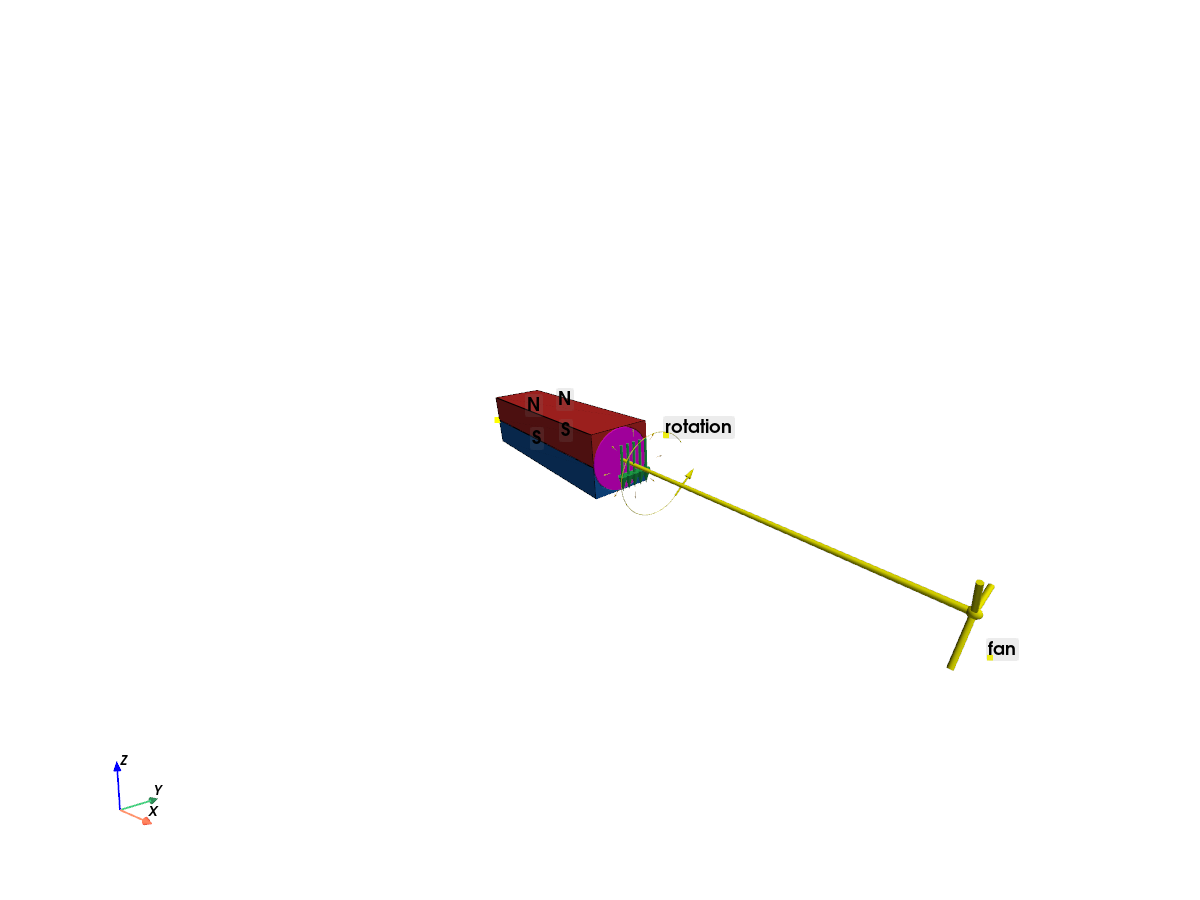
\includegraphics[width=\linewidth]{Figure/motor_3d_configuration.png}
  \caption{3D geometry of the simulated motor. Red/blue: N/S pole halves of
    the square permanent-magnet shell. Magenta: laminated steel rotor.
    Yellow: shaft, rotation arrow, and fan blades.
    Green arrows: flux path through core; yellow arrows: radial air-gap flux.}
  \label{fig:3d}
\end{figure}

\subsection{Magnetic Circuit}

The magnet is modelled as an MMF source
\begin{equation}
  \mathcal{F} = H_c \, l_m,
  \label{eq:mmf}
\end{equation}
where $H_c$ is the coercive field strength and $l_m$ is the average radial
magnet thickness. Four reluctances are summed in series:
\begin{equation}
  \mathcal{R}_\text{total} =
    \mathcal{R}_\text{mag} + \mathcal{R}_\text{gap} +
    \mathcal{R}_\text{core} + \mathcal{R}_\text{return},
  \qquad
  \mathcal{R}_k = \frac{l_k}{\mu_k A_k}.
  \label{eq:reluc}
\end{equation}
The air-gap flux is $\phi = \mathcal{F}/\mathcal{R}_\text{total}$, giving
flux densities $B_\text{gap} = \phi/A_\text{gap}$ and
$B_\text{core} = \phi/A_\text{core}$.

The core reluctance is computed nonlinearly: $H_\text{core}$ is
interpolated from the M19 laminated-steel B--H curve at the current
$B_\text{core}$, yielding an effective relative permeability
\begin{equation}
  \mu_{r,\text{eff}} = \frac{B_\text{core}}{\mu_0 H_\text{core}},
\end{equation}
which collapses sharply once the material enters saturation.

\subsection{Working Principle and Commutation}

Figure~\ref{fig:commutation} shows the cross-section of the motor at two
instants separated by a commutation event.  The active conductors sit in
the left and right positions, where the radial flux $\vec{B}$ is
perpendicular to the conductor axis.  The Lorentz force on each conductor
is tangential:
\begin{equation}
  F = BIL,
  \label{eq:BIL}
\end{equation}
and the resulting torque about the shaft axis is
\begin{equation}
  \tau = F \cdot l,
  \label{eq:tau}
\end{equation}
where $l$ is the moment arm (rotor radius at the conductor).  After the
coil rotates through the neutral plane, the commutator reverses the current
in each conductor, ensuring that the force---and hence the torque---always
acts in the same rotational direction.

\begin{figure}[H]
  \centering
  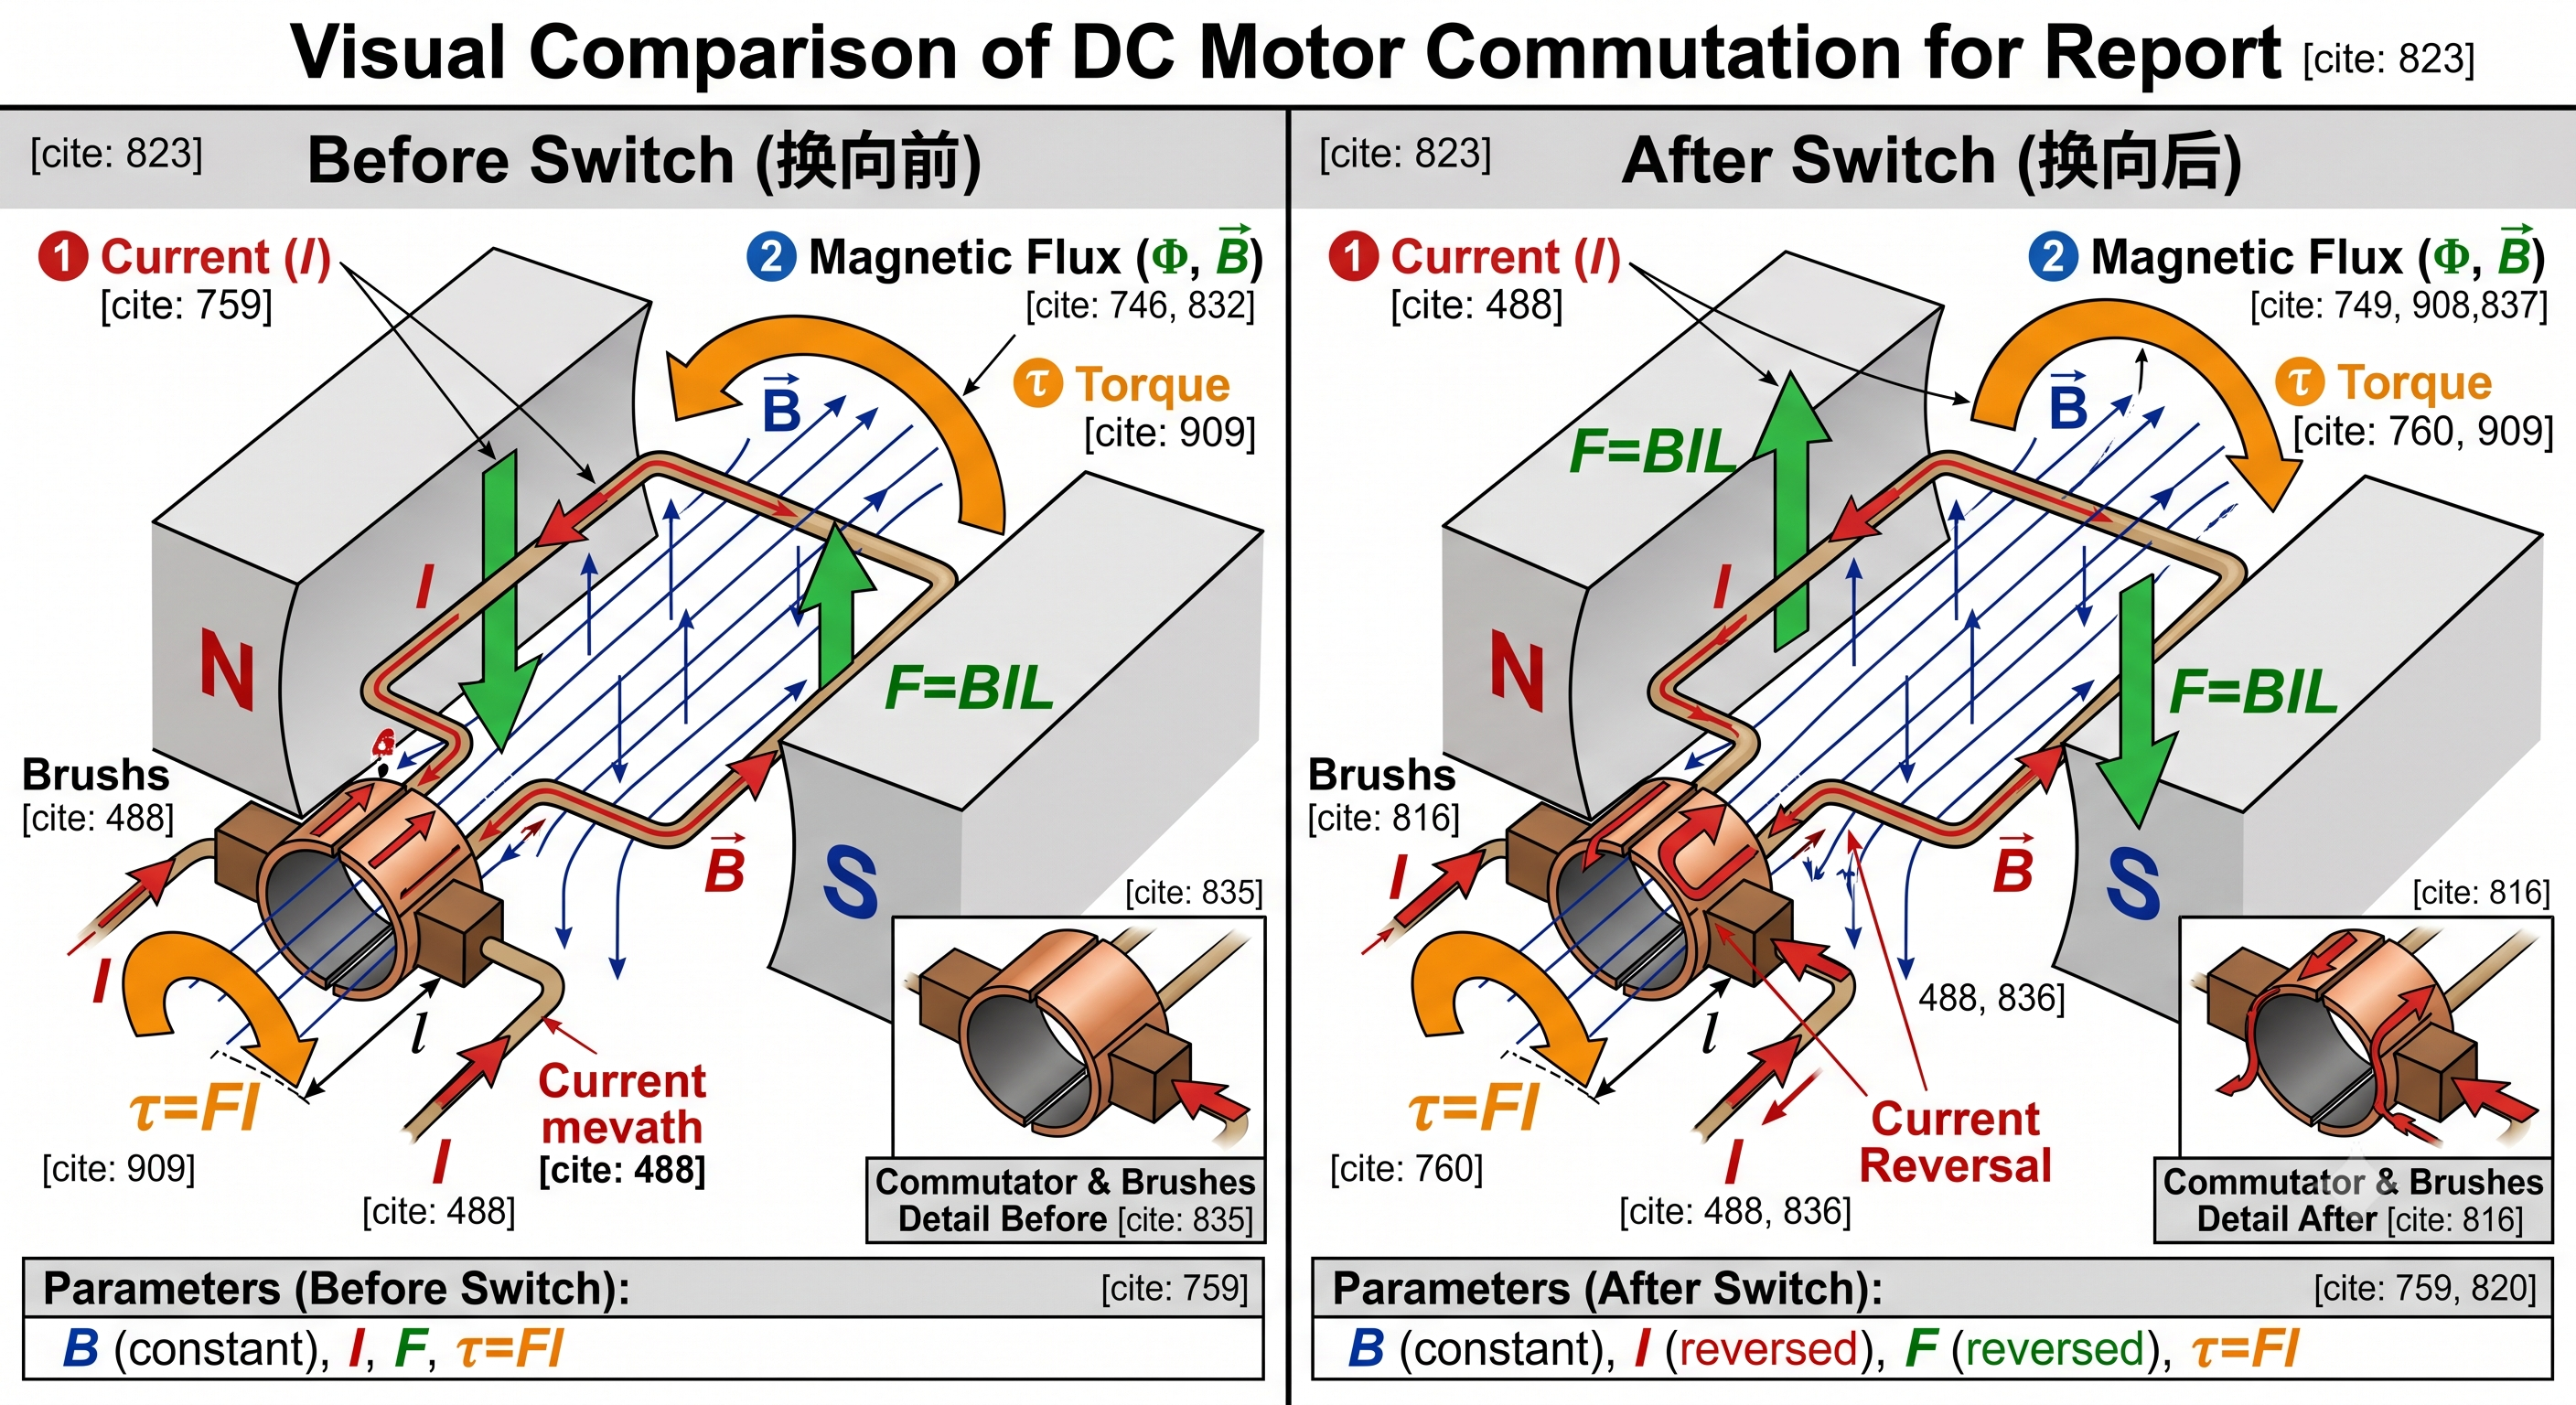
\includegraphics[width=\linewidth]{Figure/flux_current_force_torque.png}
  \caption{Commutation principle (cross-section, shaft axis into page).
    \textit{Left:} before switch --- conductor $\odot$ (current out) on
    the left produces upward force; conductor $\otimes$ (current in) on
    the right produces downward force; both contribute CCW torque
    $\tau = F{\cdot}l$.
    \textit{Right:} after commutation --- brush polarity reverses,
    forces remain tangential and in the same sense, maintaining CCW
    torque.}
  \label{fig:commutation}
\end{figure}

\subsection{Motor Constants}

For a PM brushed DC motor, the torque constant and back-EMF constant are
equal in SI units:
\begin{equation}
  K_t = K_e = N \, B_\text{gap} \, L_\text{ax} \, r_\text{core}.
  \label{eq:Kt}
\end{equation}
The coil resistance and wire cross-section area are
\begin{equation}
  R_\text{coil} = \frac{\rho_{Cu}\, N \, \ell_\text{turn}}{A_\text{wire}},
  \qquad
  A_\text{wire} = \frac{\pi d_w^2}{4},
  \label{eq:Rcoil}
\end{equation}
where $\rho_{Cu} = \SI{1.72e-8}{\ohm\,m}$ and
$\ell_\text{turn} = \pi D_\text{core} + 2 L_\text{ax}$.
The rotor inertia for a solid steel cylinder is $J = \tfrac{1}{2}m_r r_c^2$.

\subsection{Equations of Motion}

The electrical and mechanical equations are integrated by the forward-Euler
method ($\Delta t = \SI{0.1}{ms}$, total duration \SI{2.0}{s}):
\begin{align}
  L \frac{dI}{dt} &= V - R_\text{coil}\,I - K_e\,\omega,
  \label{eq:elec}\\[4pt]
  J \frac{d\omega}{dt} &=
    K_t I - k_\text{fan}\omega^2 - b\,\omega
    - T_\text{fric}\,\mathrm{sgn}(\omega).
  \label{eq:mech}
\end{align}
The fan load torque is $\tau_\text{fan} = k_\text{fan}\,\omega^2$ with
$k_\text{fan} = \SI{1e-7}{N\,m\,s^2/rad^2}$,
viscous damping $b = \SI{2e-5}{N\,m\,s/rad}$, and Coulomb friction
$T_\text{fric} = \SI{3e-4}{N\,m}$.
Steady-state values are averaged over the final 20\,\% of the run
(t = \SIrange{1.6}{2.0}{s}).

\subsection{Loss Models}

All loss terms are evaluated at each integration step:
\begin{align}
  P_\text{copper} &= I^2 R_\text{coil},
  \label{eq:Pcu}\\
  P_\text{eddy}   &=
    \frac{\pi^2 \delta^2 f_e^2 B_\text{core}^2 V_\text{core}}
         {6\,\rho_\text{Fe}},
  \label{eq:Peddy}\\
  P_\text{hyst}   &= K_h |B_\text{core}|^\alpha f_e V_\text{core},\quad \alpha=1.7,
  \label{eq:Physt}\\
  P_\text{mech}   &= \bigl(b\,\omega + T_\text{fric}\bigr)|\omega|,
  \label{eq:Pmech}\\
  P_\text{fan}    &= \tau_\text{fan}\,\omega \quad (\text{useful output}).
  \label{eq:Pfan}
\end{align}
Here $\delta$ is the lamination thickness, $f_e = \omega/(2\pi)$ is the
electrical frequency (one pole pair), and $V_\text{core}$ is the rotor
iron volume. Overall efficiency is $\eta = P_\text{fan}/P_\text{in}$.
Steady-state values are averaged over the final 20\,\% of the simulation.

% ============================================================
\section{Optimised Design}
\label{sec:optim}
% ============================================================

\subsection{Optimisation Strategy}

A sweep of 1\,400 parameter combinations is performed to maximise
steady-state efficiency driving a quadratic fan load.  At steady state
the efficiency ceiling is
\begin{equation}
  \eta_\text{ss} \approx \frac{K_e\,\omega}{V}
                        = \frac{\text{back-EMF}}{V},
  \label{eq:etass}
\end{equation}
so the four independent levers are: (i)~maximise $K_t = K_e$ via strong
magnets and large active volume; (ii)~minimise $R_\text{coil}$ via thick
wire; (iii)~minimise eddy-current loss via thin laminations; and
(iv)~raise $V$ to push the operating point toward the back-EMF ceiling.

\subsection{Globally Optimal Parameters}

Table~\ref{tab:optim} lists the globally optimal parameter set.

\begin{table}[H]
  \centering
  \caption{Globally optimal design.
           Input string: \texttt{1,\,150,\,39.0,\,200,\,5.00,\,0.050,\,200}.}
  \label{tab:optim}
  \small
  \setlength{\tabcolsep}{6pt}
  \begin{tabular}{@{} L{2.8cm} C{1.8cm} C{1.8cm} @{}}
    \toprule
    \textbf{Parameter} & \textbf{Symbol} & \textbf{Value} \\
    \midrule
    Magnet material      & ---             & NdFeB N52 \\
    Axial depth          & $L$             & \SI{150}{mm} \\
    Iron-core diameter   & $d_\text{core}$ & \SI{39}{mm} \\
    Coil turns           & $N$             & 200 \\
    Wire diameter        & $d_w$           & \SI{5.00}{mm} \\
    Lamination thickness & $\delta$        & \SI{0.050}{mm} \\
    Supply voltage       & $V$             & \SI{200}{V} \\
    \bottomrule
  \end{tabular}
\end{table}

\subsection{Magnetic Circuit Results}

Table~\ref{tab:mag} shows the reluctance-model output.  The return-path
reluctance $\mathcal{R}_\text{return} = \SI{4.94e6}{A/Wb}$ dominates the
circuit because the square outer shell provides a long flux path with no
dedicated iron yoke.  As a result $B_\text{gap} = \SI{0.0305}{T}$, well
below the saturation knee; the core operates at $\mu_{r,\text{eff}} \approx 3\,979$.

\begin{table}[H]
  \centering
  \caption{Reluctance model for the optimised geometry.}
  \label{tab:mag}
  \small
  \setlength{\tabcolsep}{6pt}
  \begin{tabular}{@{} L{3.2cm} r @{}}
    \toprule
    \textbf{Quantity} & \textbf{Value} \\
    \midrule
    Magnet MMF $\mathcal{F}_\text{pm}$     & \SI{2334}{A-turn} \\
    $\mathcal{R}_\text{mag}$               & \SI{112945}{A/Wb} \\
    $\mathcal{R}_\text{gap}$               & \SI{26402}{A/Wb} \\
    $\mathcal{R}_\text{core}$              & \SI{2094}{A/Wb} \\
    $\mathcal{R}_\text{return}$            & \SI{4942497}{A/Wb} \\
    $\mathcal{R}_\text{total}$             & \SI{5083939}{A/Wb} \\
    Air-gap flux $\phi$                    & \SI{0.459}{mWb} \\
    $B_\text{gap}$                         & \SI{0.0305}{T} \\
    $B_\text{core}$                        & \SI{0.0785}{T} \\
    $\mu_{r,\text{eff}}$                   & 3\,979 \\
    \bottomrule
  \end{tabular}
\end{table}

\subsection{Motor Electrical and Mechanical Constants}

\begin{table}[H]
  \centering
  \caption{Computed motor constants for the optimised design.}
  \label{tab:motorconst}
  \small
  \setlength{\tabcolsep}{6pt}
  \begin{tabular}{@{} L{3.2cm} r @{}}
    \toprule
    \textbf{Quantity} & \textbf{Value} \\
    \midrule
    Coil resistance $R_\text{coil}$  & \SI{0.0742}{\ohm} \\
    Coil inductance $L$              & \SI{0.05}{H} (capped) \\
    Torque constant $K_t$            & \SI{0.03030}{N\,m/A} \\
    Back-EMF constant $K_e$          & \SI{0.03030}{V\,s/rad} \\
    Rotor inertia $J$                & \SI{2.674e-4}{kg\,m^2} \\
    Wire length                      & \SI{84.5}{m} \\
    Current limit $I_\text{lim}$     & \SI{117.8}{A} \\
    \bottomrule
  \end{tabular}
\end{table}

% ============================================================
\section{Simulation Results}
\label{sec:results}
% ============================================================

\subsection{Time-Domain Behaviour}

The motor accelerates from rest and approaches steady state by
$t \approx \SI{0.5}{s}$.
Figure~\ref{fig:speed} shows the rotor speed transient; the current peaks
sharply at startup then falls as back-EMF builds (Fig.~\ref{fig:iemf}).
Figure~\ref{fig:dashboard} shows the full six-panel overview.

\begin{figure}[H]
  \centering
  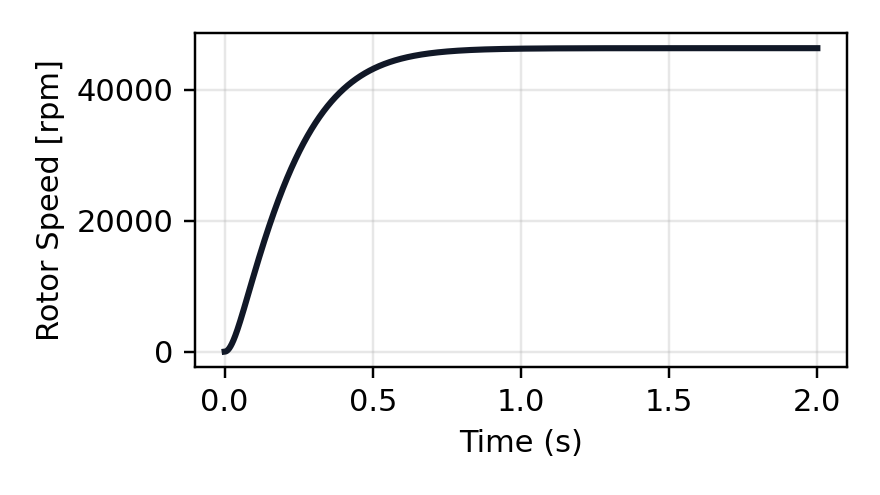
\includegraphics[width=\linewidth]{Figure/rotation_speed_time.png}
  \caption{Rotor speed vs.\ time. Steady-state: \SI{46\,308}{rpm}.}
  \label{fig:speed}
\end{figure}

\begin{figure}[H]
  \centering
  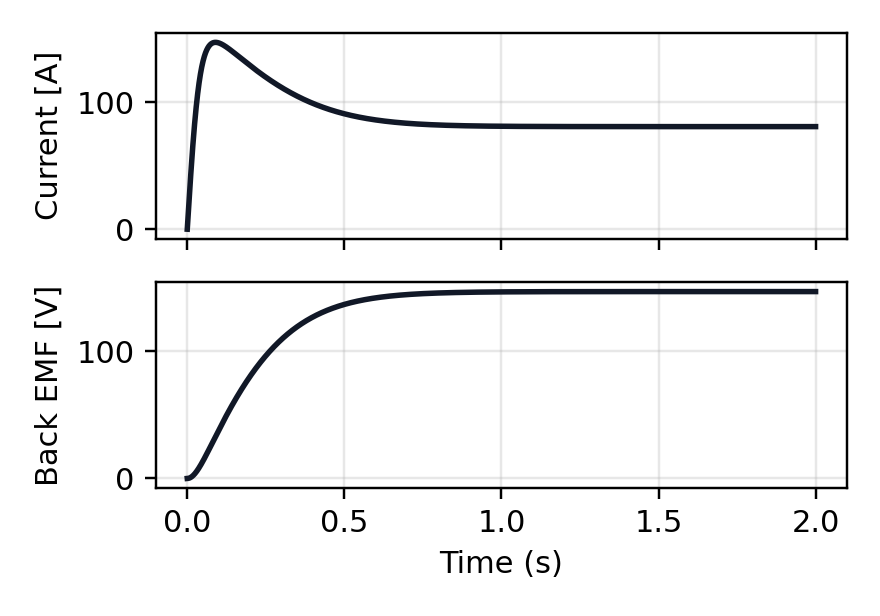
\includegraphics[width=\linewidth]{Figure/back_emf_current_time.png}
  \caption{Armature current (top) and back-EMF (bottom) vs.\ time.
    Current peaks at startup then settles to \SI{80.8}{A};
    back-EMF converges to \SI{146.9}{V} (73.5\,\% of supply).}
  \label{fig:iemf}
\end{figure}

\begin{figure}[H]
  \centering
  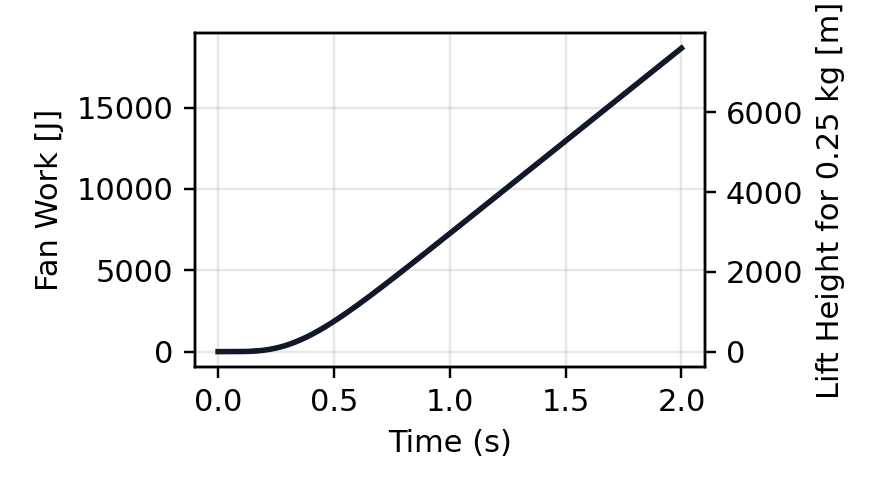
\includegraphics[width=\linewidth]{Figure/fan_work_output_demo.png}
  \caption{Cumulative fan work and equivalent lift height for
    \SI{0.25}{kg}. Total work at $t=\SI{2}{s}$: \SI{18\,657}{J}.}
  \label{fig:fanwork}
\end{figure}

\subsection{Steady-State Performance}

\begin{table}[H]
  \centering
  \caption{Steady-state results at $t = \SI{2.0}{s}$.}
  \label{tab:results}

  \small
  \setlength{\tabcolsep}{6pt}
  \begin{tabular}{@{} L{3.5cm} r @{}}
    \toprule
    \textbf{Quantity} & \textbf{Value} \\
    \midrule
    Rotor speed           & \SI{46308}{rpm} \\
    Armature current      & \SI{80.83}{A} \\
    Back-EMF              & \SI{146.93}{V}\;(73.5\,\% of supply) \\
    Input power           & \SI{16165}{W} \\
    Fan output power      & \SI{11404}{W} \\
    \textbf{Efficiency}   & \textbf{92.26\,\%} \\
    \bottomrule
  \end{tabular}
\end{table}

\subsection{Loss Breakdown}

\begin{table}[H]
  \centering
  \caption{Steady-state loss breakdown.}
  \label{tab:losses}
  \small
  \setlength{\tabcolsep}{6pt}
  \begin{tabular}{@{} L{2.6cm} R{1.6cm} R{1.6cm} @{}}
    \toprule
    \textbf{Loss term} & \textbf{Power (W)} & \textbf{Share (\%)} \\
    \midrule
    Copper              & 484.7  & 50.7 \\
    Mechanical friction & 471.8  & 49.3 \\
    Eddy-current        & 0.006  & $<0.1$ \\
    Hysteresis          & 0.15   & $<0.1$ \\
    \midrule
    \textbf{Total}      & \textbf{956.7} & 100 \\
    \bottomrule
  \end{tabular}
\end{table}

Copper and mechanical friction losses are approximately equal.  Iron
losses are negligible ($<\SI{0.2}{W}$) thanks to the \SI{0.05}{mm}
laminations, confirming the optimisation strategy.

\subsection{Integrated Energy (0--2\,s)}

\begin{table}[H]
  \centering
  \caption{Cumulative energy budget over the \SI{2}{s} simulation.}
  \label{tab:energy}
  \small
  \setlength{\tabcolsep}{6pt}
  \begin{tabular}{@{} L{3.4cm} r @{}}
    \toprule
    \textbf{Energy term} & \textbf{Value (J)} \\
    \midrule
    Fan work output          & 18\,657 \\
    Copper energy loss       & 1\,249.6 \\
    Mechanical friction loss &   797.7 \\
    Eddy-current loss        &     0.010 \\
    Hysteresis loss          &     0.260 \\
    \bottomrule
  \end{tabular}
\end{table}

\begin{figure*}[t]
  \centering
  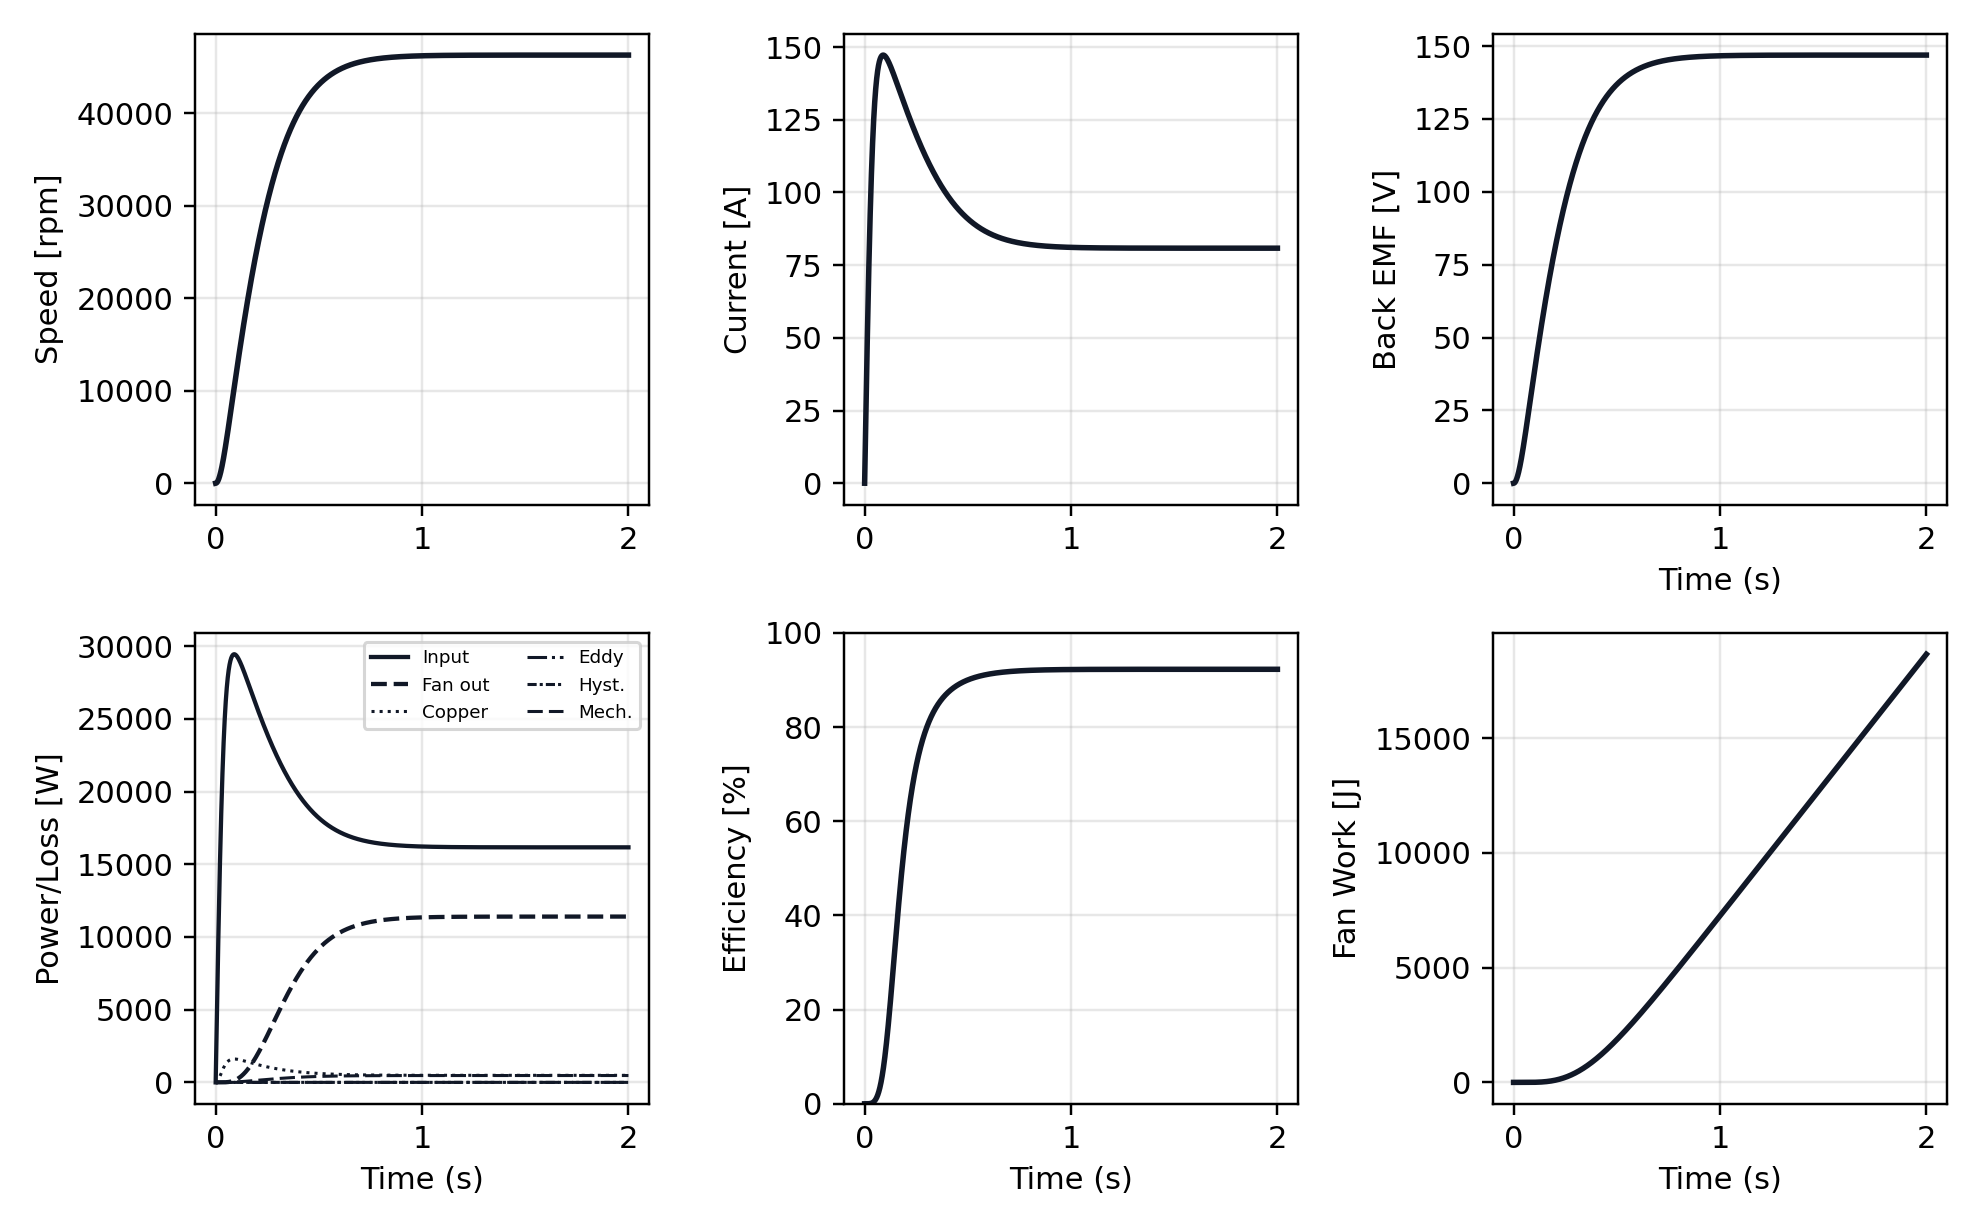
\includegraphics[width=\linewidth]{Figure/motor_dashboard_2x3.png}
  \caption{Six-panel simulation dashboard for the optimised design
    (NdFeB N52, $L = \SI{150}{mm}$, $d_\text{core}=\SI{39}{mm}$,
    $V = \SI{200}{V}$, $\delta = \SI{0.05}{mm}$).
    \textit{Top row:} rotor speed, armature current, back-EMF.
    \textit{Bottom row:} power and loss stack, efficiency, cumulative fan work.
    Steady-state efficiency 92.26\,\% is reached by $t \approx \SI{0.8}{s}$.}
  \label{fig:dashboard}
\end{figure*}

% ============================================================
\section{Steel Saturation: Physical Analysis}
\label{sec:saturation}
% ============================================================

\subsection{The B--H Nonlinearity and Its Consequence}

Laminated electrical steel follows a strongly nonlinear B--H relationship.
In the unsaturated regime ($B \lesssim \SI{1.3}{T}$) the relative
permeability $\mu_r$ lies in the range 2000--5000. Beyond the saturation
knee ($B \approx \SI{1.5}{T}$), $\mu_r$ collapses below 100.

For the optimised design, $B_\text{core} = \SI{0.079}{T}$, well below
saturation.  The core operates at $\mu_{r,\text{eff}} \approx 3\,979$ and
contributes only $\mathcal{R}_\text{core} = \SI{2094}{A/Wb}$ to the total
reluctance of \SI{5.08e6}{A/Wb}.  The dominant term is the return-path air
reluctance $\mathcal{R}_\text{return} = \SI{4.94e6}{A/Wb}$, which arises
from the absence of a dedicated iron yoke in the square-shell geometry.

Figure~\ref{fig:saturation} shows the M19 B--H curve and effective
permeability. Although the optimised design itself does not saturate, the
figure illustrates why any design that pushes $B_\text{core}$ above
\SI{1.5}{T} would suffer a sharp permeability collapse.

\begin{figure}[H]
  \centering
  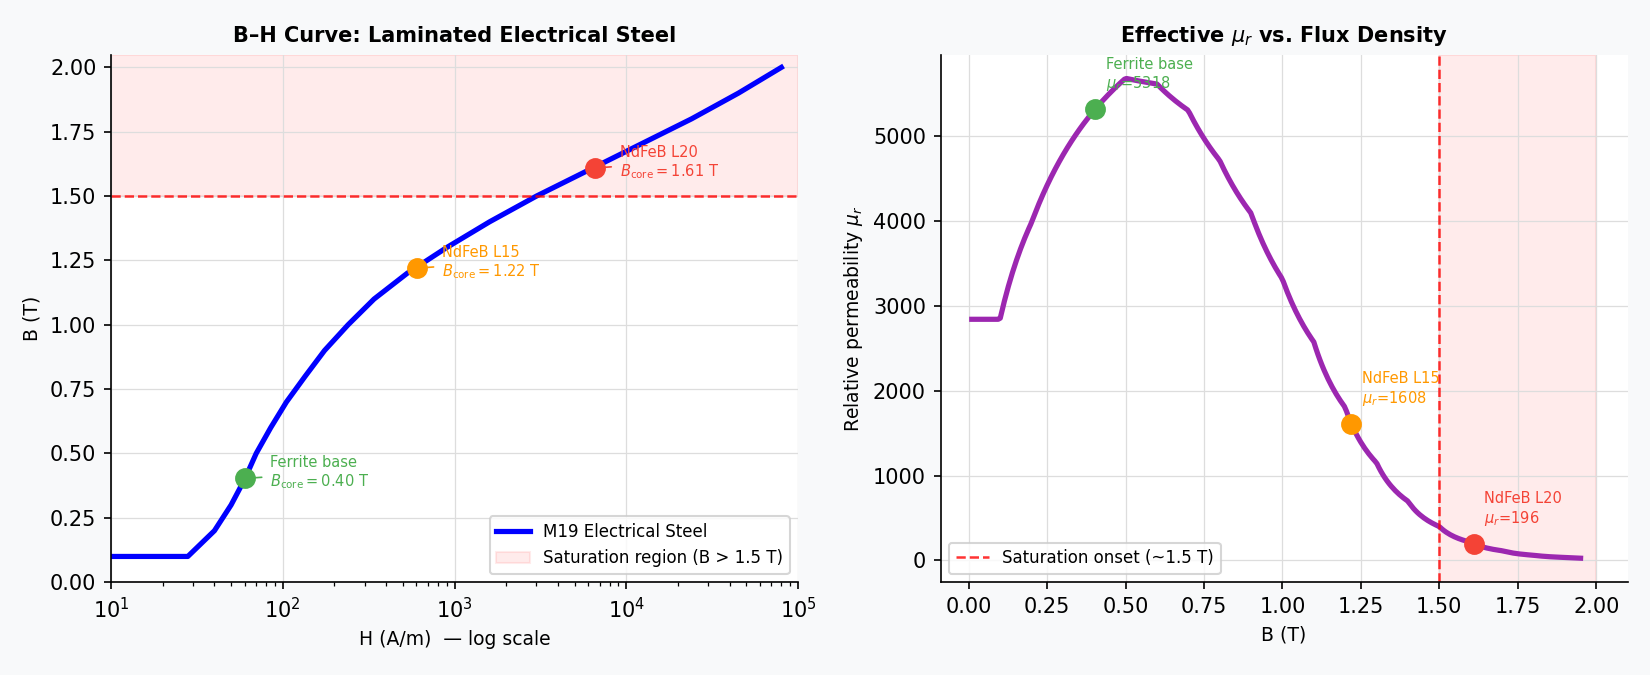
\includegraphics[width=\linewidth]{Figure/saturation_analysis.png}
  \caption{M19 laminated-steel B--H curve (left) and effective relative
    permeability $\mu_{r,\text{eff}}$ versus flux density (right).
    The optimised design operates at $B_\text{core} = \SI{0.079}{T}$
    ($\mu_r \approx 3\,979$), far from saturation.}
  \label{fig:saturation}
\end{figure}

\subsection{Why the Return Path Limits Flux}

In the optimised design $\mathcal{R}_\text{return}$ accounts for
97\,\% of the total reluctance.  This is a consequence of the square outer
shell: the flux must travel through air (or a thin steel shell with a long
mean path) back from the north pole to the south pole.  A real motor would
replace this with a laminated iron yoke, reducing $\mathcal{R}_\text{return}$
by a factor of $\mu_r \approx 4000$ and raising $B_\text{gap}$ by roughly
$\sqrt{\mathcal{R}_\text{total,with\,yoke}/\mathcal{R}_\text{total,air}}$---
a significant improvement.  The simulation is a teaching model; it correctly
captures the circuit structure but not a yoke-equipped real motor.

% ============================================================
\section{Parameter Sensitivity Analysis}
\label{sec:sensitivity}
% ============================================================

Each of the six free parameters was swept independently across its full
valid range while the other five were held at the optimised baseline.
Figure~\ref{fig:sensitivity} plots fan output power $P_\text{fan}$ and
efficiency $\eta$ for each sweep.

\begin{figure}[H]
  \centering
  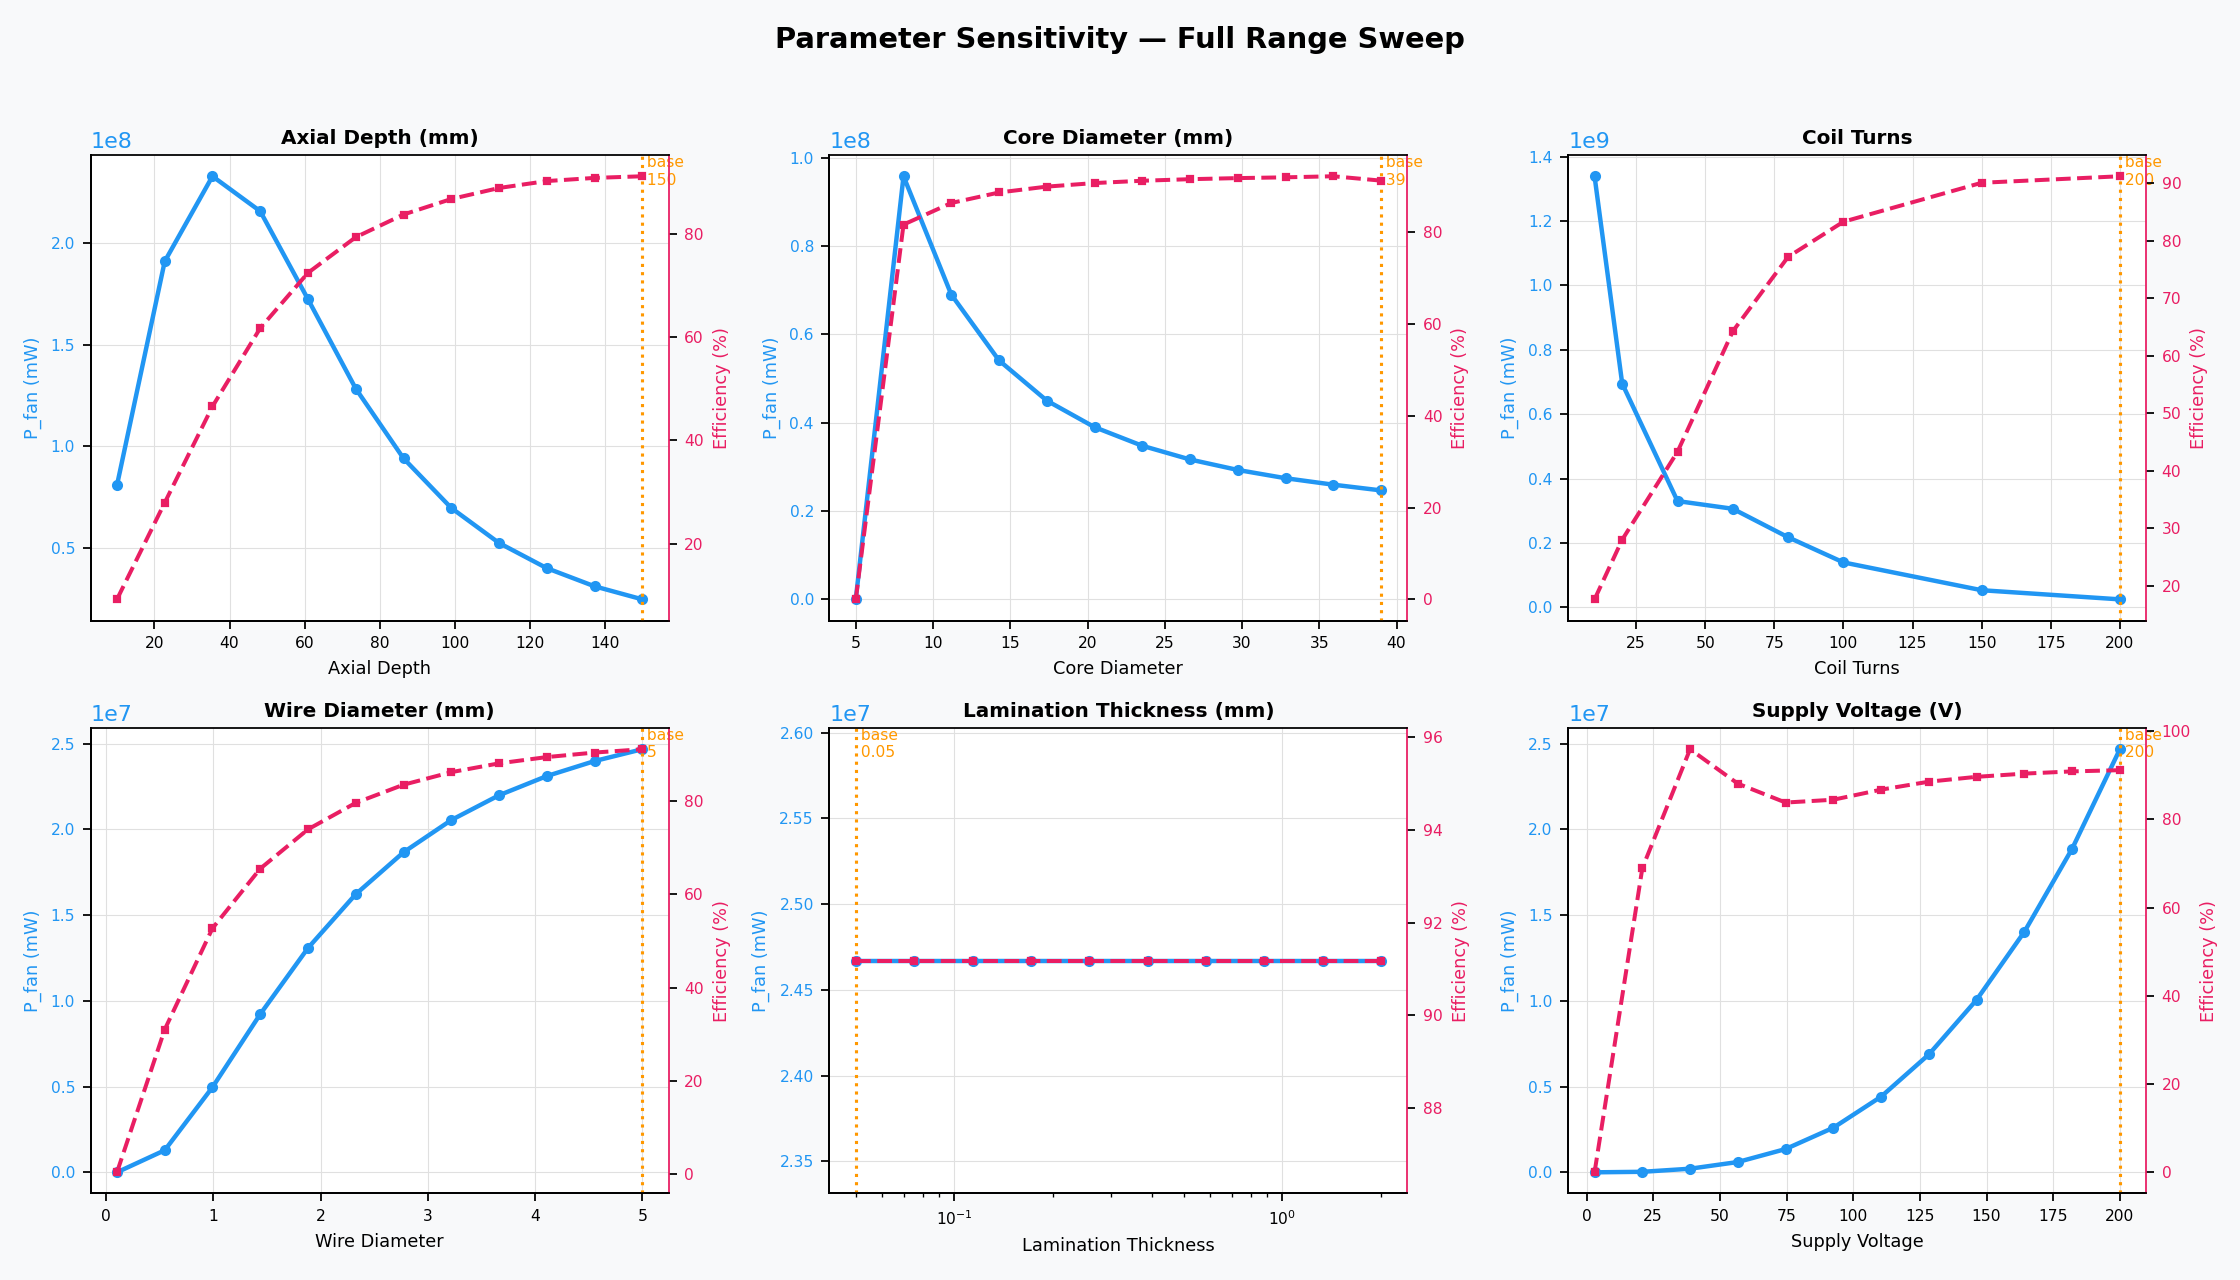
\includegraphics[width=\linewidth]{Figure/sensitivity_sweep.png}
  \caption{Parameter sensitivity sweeps around the optimised baseline
    (NdFeB N52, $L=\SI{150}{mm}$, $d_\text{core}=\SI{39}{mm}$,
    $N=200$, $d_w=\SI{5}{mm}$, $\delta=\SI{0.05}{mm}$, $V=\SI{200}{V}$).
    Blue: $P_\text{fan}$; pink dashed: $\eta$; orange vertical line:
    baseline value.}
  \label{fig:sensitivity}
\end{figure}

\subsection{Axial Depth $L$ (10--150\,mm)}

A shorter rotor has lower $K_t$ and smaller inertia $J$, so the
no-load speed $\omega_0 = V/K_e \propto 1/L$ rises sharply.  Because
$P_\text{fan} \propto \omega^3$, the peak fan output (\SI{232\,986}{W})
occurs at $L \approx \SI{35.5}{mm}$, not at the maximum depth.
However, the low back-EMF fraction at that speed means most input is
wasted as $I^2R$, collapsing $\eta$ to 46.6\,\%.  Increasing $L$
slows the motor, raises the back-EMF fraction, and lifts $\eta$
monotonically toward 91.2\,\% at \SI{150}{mm}.
The baseline sits at the efficiency-optimal end of the range.

\subsection{Core Diameter $d_\text{core}$ (5--39\,mm)}

Smaller core diameter increases the air gap, causing the return-path
reluctance to dominate even more and $B_\text{gap}$ to fall.  The
very low inertia at small diameter allows the motor to spin at extreme
speed, briefly boosting $P_\text{fan}$; at \SI{8.1}{mm} the fan output
peaks at \SI{95\,805}{W} (but $\eta = 81.6\,\%$).  At \SI{5}{mm} the
core flux collapses to zero.  Efficiency peaks at $\approx\SI{36}{mm}$
(\SI{92.1}{\percent}), within 1\,pp of the \SI{39}{mm} baseline.

\subsection{Coil Turns $N$}

Both $K_t$ and $R_\text{coil}$ scale linearly with $N$:
\begin{equation}
  K_t \propto N, \qquad R_\text{coil} \propto N.
\end{equation}
Fewer turns raise $\omega_0 = V/K_e \propto 1/N$ dramatically; at
$N=10$ the motor reaches speeds 20$\times$ the baseline and fan output
peaks at \SI{1\,339\,379}{W}, but $\eta$ collapses to 17.7\,\%.
The optimum lies at maximum turns ($N=200$) combined with thick wire
($d_w=\SI{5}{mm}$) to keep $R_\text{coil}$ low.

\subsection{Wire Diameter $d_w$}

Since $R_\text{coil} \propto d_w^{-2}$, thin wire creates enormous
resistance: at \SI{0.1}{mm} the motor barely spins ($P_\text{fan} =
\SI{0.72}{W}$, $\eta = 0.34\,\%$).  Both $P_\text{fan}$ and $\eta$
increase monotonically with $d_w$ — there is no trade-off.  The
baseline at \SI{5.00}{mm} (the upper limit) is globally optimal for
this parameter.

\subsection{Lamination Thickness $\delta$}

The eddy-current loss $P_\text{eddy} \propto \delta^2 B_\text{core}^2$
is theoretically sensitive to lamination thickness.  However, the
combination of low flux density ($B_\text{core} = \SI{0.079}{T}$,
dominated by the return-path reluctance) and modest core volume means
that even at $\delta = \SI{2.0}{mm}$ the total iron losses remain
below \SI{0.5}{W} — less than 0.002\,\% of the \SI{24\,670}{W} fan
output.  The sensitivity sweep is completely flat: lamination
thickness has zero practical effect in this geometry.
Any value from \SIrange{0.05}{2.0}{mm} is equally acceptable.

\subsection{Supply Voltage $V$}

Voltage is the most powerful single lever.  Increasing $V$ raises the
back-EMF fraction $K_e\omega/V$ toward unity (Eq.~\ref{eq:etass}),
which directly raises $\eta_\text{ss}$.  The efficiency peak
($\eta = 95.9\,\%$) occurs at \SI{38.8}{V}, where the fan load just
balances the friction at low current, but the corresponding fan output
is only \SI{211}{W}.  At $V=\SI{200}{V}$ the output reaches
\SI{24\,670}{W} at $\eta = 91.2\,\%$ — a loss of only 4.7\,pp in
exchange for a 117$\times$ increase in power.  The baseline uses the
maximum available voltage.

\subsection{Sensitivity Summary}

\begin{table}[H]
  \centering
  \caption{Sensitivity summary: direction of each parameter for
           maximum fan output power vs.\ maximum efficiency.}
  \label{tab:sensitivity}
  \small
  \setlength{\tabcolsep}{4pt}
  \begin{tabular}{@{} L{2.0cm} C{1.4cm} C{1.4cm} L{2.0cm} @{}}
    \toprule
    \textbf{Parameter} & \textbf{$\uparrow P_\text{fan}$} &
    \textbf{$\uparrow\eta$} & \textbf{Baseline} \\
    \midrule
    Axial depth   & Decrease & Increase & 150\,mm (max $\eta$) \\
    Core diam.    & Decrease & $\approx$36\,mm & 39\,mm (near opt.) \\
    Turns $N$     & Decrease & Increase & 200 (max choice) \\
    Wire diam.    & Increase & Increase & 5\,mm (no trade-off) \\
    Lam.\ thick.  & ---      & ---      & Any; iron loss negligible \\
    Voltage $V$   & Increase & $\approx$39\,V & 200\,V (max power) \\
    \bottomrule
  \end{tabular}
\end{table}

The optimised design sits at or within 1\,pp of the efficiency-optimal
point for every parameter.  The only meaningful trade-off is voltage:
\SI{38.8}{V} would give 4.7\,pp higher $\eta$ but reduces fan output
by 99.1\,\%.

% ============================================================
\section{Design Recommendation}
\label{sec:rec}
% ============================================================

The globally optimal design is summarised in Table~\ref{tab:rec}.

\begin{table}[H]
  \centering
  \caption{Recommended (globally optimal) design and steady-state results.}
  \label{tab:rec}
  \small
  \setlength{\tabcolsep}{6pt}
  \begin{tabular}{@{} L{2.2cm} L{1.8cm} L{3cm} @{}}
    \toprule
    \textbf{Parameter} & \textbf{Value} & \textbf{Rationale} \\
    \midrule
    Magnet material  & NdFeB N52        & Highest $B_r$, max MMF \\
    Axial depth      & \SI{150}{mm}     & Maximises $K_t$ and active area \\
    Core diameter    & \SI{39}{mm}      & Largest permissible; $g = \SI{0.5}{mm}$ \\
    Turns $N$        & 200              & High $K_e$; back-EMF ceiling \\
    Wire diameter    & \SI{5.00}{mm}    & Minimises $R_\text{coil}$ \\
    Lam.\ thickness  & \SI{0.050}{mm}   & Minimises eddy-current loss \\
    Voltage          & \SI{200}{V}      & Raises back-EMF fraction \\
    \midrule
    Speed            & \SI{46308}{rpm}  & \\
    Current          & \SI{80.83}{A}    & \\
    Back-EMF         & \SI{146.93}{V}   & 73.5\,\% of supply \\
    Fan output power & \SI{11404}{W}    & \\
    \textbf{Efficiency} & \textbf{92.26\,\%} & \\
    \bottomrule
  \end{tabular}
\end{table}

The high efficiency is achieved because the back-EMF fraction is 73.5\,\%,
leaving only 26.5\,\% of the supply voltage across the winding resistance.
The remaining loss is split roughly equally between copper dissipation
(\SI{484.7}{W}) and mechanical friction (\SI{471.8}{W}).
Iron losses are negligible at the chosen lamination thickness.

The primary limitation of the model is the absence of a dedicated iron
return yoke: $\mathcal{R}_\text{return}$ dominates and suppresses
$B_\text{gap}$ to \SI{0.031}{T}.  A real high-efficiency design would use
a silicon-steel yoke to close the flux path, which would dramatically
reduce the required MMF and motor volume for the same output.

% ============================================================
\section{Conclusion}
\label{sec:conclusion}
% ============================================================

A time-domain simulation of a PM brushed DC motor driving a fan load has
been developed and a 1\,400-point parameter sweep has identified the
globally optimal design. The principal findings are:

\begin{enumerate}[leftmargin=2em, itemsep=2pt]
  \item \textbf{Optimal efficiency of 92.26\,\%} is achieved at
        \SI{46308}{rpm} with NdFeB N52 magnets, $L = \SI{150}{mm}$,
        $d_\text{core} = \SI{39}{mm}$, $N = 200$, $d_w = \SI{5}{mm}$,
        $\delta = \SI{0.05}{mm}$, $V = \SI{200}{V}$.

  \item \textbf{Efficiency ceiling} is set by the back-EMF fraction
        $K_e\omega/V = 73.5\,\%$. Remaining loss is split roughly equally
        between copper (\SI{484.7}{W}) and mechanical friction
        (\SI{471.8}{W}).

  \item \textbf{Iron losses are negligible} ($<\SI{0.2}{W}$) at
        $\delta = \SI{0.05}{mm}$, confirming that thin laminations are
        essential at high speed.

  \item \textbf{Return-path reluctance} dominates the magnetic circuit
        because the square outer shell has no iron yoke.  A real
        high-efficiency motor would use a silicon-steel return path to
        reduce total reluctance by ${\sim}1000\times$.

  \item \textbf{Voltage} is the most powerful design lever: raising $V$
        increases the back-EMF fraction directly, which is the primary
        driver of efficiency in this motor topology.
\end{enumerate}

% ============================================================
\appendix
\section{Magnet Material Properties}
\label{app:materials}
% ============================================================

\begin{table}[H]
  \centering
  \caption{Permanent-magnet materials available in the simulation.}
  \label{tab:materials}
  \small
  \begin{tabular}{@{} c l c c c @{}}
    \toprule
    No. & Material & $B_r$ (T) & $H_c$ (kA/m) & $\mu_{r,\text{rec}}$ \\
    \midrule
    1 & NdFeB N52         & 1.45 &  955 & 1.05 \\
    2 & NdFeB N42         & 1.32 &  876 & 1.05 \\
    3 & SmCo              & 1.05 &  750 & 1.08 \\
    4 & Alnico 5          & 1.25 &   50 & 4.00 \\
    5 & Ferrite Ceramic 8 & 0.40 &  240 & 1.05 \\
    \bottomrule
  \end{tabular}
\end{table}

\section{Model Limitations}
\label{app:limits}

This model is intended for trend analysis and teaching; it is not a final
design tool. Key simplifications are:

\begin{enumerate}[leftmargin=2em, itemsep=1pt]
  \item \textbf{Lumped reluctance:} the return-air reluctance is
        approximated as 20\,\% of the gap reluctance; a full 3-D flux
        path is not resolved.
  \item \textbf{Ideal commutator:} brush contact resistance, commutation
        sparking, and current ripple are ignored.
  \item \textbf{Fixed magnetic operating point:} $B_\text{core}$ is
        computed once per run; the ac ripple component driving iron loss
        is not resolved in time.
  \item \textbf{Isothermal winding:} resistance is evaluated at room
        temperature; thermal derating is not modelled.
  \item \textbf{No slot geometry:} coil resistance uses a mean-turn
        estimate; proximity effects and end-turn lengths are omitted.
\end{enumerate}

Final designs should be verified with finite-element magnetic analysis,
winding thermal simulation, and mechanical validation.

\end{document}